\documentclass[11pt]{article}
\usepackage[utf8]{inputenc}
\usepackage{amsmath,amsthm,amsfonts,amssymb,amscd}
\usepackage{multirow,booktabs}
\usepackage[table]{xcolor}
\usepackage{fullpage}
\usepackage{lastpage}
\usepackage{enumitem}
\usepackage{fancyhdr}
\usepackage{mathrsfs}
\usepackage{array}
\usepackage{wrapfig}
\usepackage{setspace}
\usepackage{calc}
\usepackage{graphicx}
\usepackage{multicol}
\usepackage{cancel}
\usepackage[retainorgcmds]{IEEEtrantools}
\usepackage[margin=3cm]{geometry}
\usepackage{amsmath}
\usepackage[most]{tcolorbox} \usepackage{xcolor}

\graphicspath{{./images/}}

\newlength{\tabcont}
\setlength{\parindent}{0.0in} \setlength{\parskip}{0.05in} \usepackage{empheq} \usepackage{framed}


\colorlet{shadecolor}{orange!15}
\parindent 0in
\parskip 12pt \geometry{margin=1in, headsep=0.25in} \theoremstyle{definition}

\begin{document}

\thispagestyle{empty}

\newtheorem{definition}{Definition}[section]
\newtheorem{anmk}{Anmerkung}[section]
\newtheorem{bsp}{Beispiel}[section]
\newtheorem{aufgabe}{Aufgabe}[section]

\newcommand{\N}{\mathbb{N}}
\newcommand{\Z}{\mathbb{Z}}
\newcommand{\R}{\mathbb{R}}

\begin{center}
  {\LARGE \bf Web Engineering I}\\
  {\Large Web Engineering I}\\
  WS 2024
\end{center}

\section{Übung -- 15.10.2024}
\subsection{Aufgabe 1.1}
Die grobe Timeline des Internets sieht folgendermaßen aus:
\begin{itemize}
  \item 1968: Entwicklung des Arpanets durch Forscher des MIT und des US-Verteidigungsministeriums
  \item 1983: Einführung des TCP/IP-Protokolls
  \item 1989: Entwicklung des World Wide Web durch Tim Berners-Lee
  \item 1993: Einführung des ersten Web-Browsers Mosaic (neben dem "World Wide Web" Browser von Berners-Lee)
\end{itemize}

\subsection{Aufgabe 1.2}
Wichtige Entwicklungen und Ereignisse des Internets:
\begin{itemize}
  \item 1972: Erstes E-Mail-Programm wird durch Ray Tomlinson entwickelt
  \item 1977: TCP/IP wird auf Basis des CYCLADES-Netzwerks entwickelt
  \item 1984: Erstmalige Verwendung des Domain Name Systems (DNS)
  \item 1986: Die ersten .de Domains werden registriert
  \item 1998: Google wird gegründet
  \item 1999: Eine Million .de Domains werden registriert
  \item 2001: Wikipedia wird gegründet
\end{itemize}

\subsection{Aufgabe 1.3}
Ein Pionier des Internets ist Teus Hagen, unter anderem an der Entwicklung des TCP/IP-Protokolls beteiligt
war.

\subsection{Aufgabe 1.4}
\begin{itemize}
  \item ISOC: Internet Society. Sie ist eine internationale Organisation, die sich für die Entwicklung und
        Standardisierung des Internets einsetzt.
  \item W3C: World Wide Web Consortium. Es ist eine internationale Organisation, die sich für die Entwicklung und
        Standardisierung des World Wide Web einsetzt.
  \item ICANN: Internet Corporation for Assigned Names and Numbers. Sie ist eine internationale Organisation, die sich
        um die Vergabe von Domainnamen und IP-Adressen kümmert.
\end{itemize}

\section{Übung -- 22.10.2024}
\begin{aufgabe}
  Was ist der Unterschied zwischen einem (Internet) Dienst und einem Protokoll?

  Ein Dienst stellt stellt eine bestimmte Funktionalität dar, während ein Protokoll zur Kommunikation mit einem Dienst
  verwendet wird.

  Beispiele für Dienste: FTP-Server, E-Mail-Server, Web-Server

  Beispiele für Protokolle: HTTP(S), SMTP, FTP
\end{aufgabe}

\begin{aufgabe}
  Was sind Schichtenmodelle?

  Schichtenmodelle beschreiben den technischen Aufbau der Netzwerkkommunikation und teilen Datenpakete ist verschiedene
  Schichten auf.

  Die bekanntesten Schichtenmodelle sind das ISO/OSI-Modell und das TCP/IP-Modell. Diese unterscheiden sich darin, dass
  das TCP/IP Modell im wesentlichen die drei Anwendungsschichten in einer Schicht vereint und die ersten beiden Schichten
  werden ebenfalls kombiniert. Somit beinhaltet das TCP/IP-Modell nur vier der sieben Schichten des ISO/OSI-Modells.

  Protokolle auf Transportebene: TCP, UDP

  Protokolle auf Anwendungsebene: HTTP, FTP
\end{aufgabe}

\begin{aufgabe}
  Warum werden die Daten beim OSI-Referenzmodell von Schicht 1 zu Schicht 7 weniger?

  Dadurch, dass jede Schicht ihre eigenen Header und Tailer anhängt, wird mit jeder Schicht mehr "drumherum" gebaut
  und somit sind die Datenpakete bei Schicht 7 größer als bei Schicht 1.
\end{aufgabe}

\begin{aufgabe}
  Auf welcher Schicht ist Wireless LAN (WLAN) angesiedelt?

  WLAN ist auf der Schicht 1 (Bitübertragungs-Schicht) angesiedelt.

  Wi-Fi 4, 5 und 6 sind Standards für WLAN, die jeweils einen IEEE 802.11-Standard darstellen. Dabei ist Wi-Fi 4 gleich
  dem 802.11n Standard, Wi-Fi 5 entspricht 802.11ac, Wi-Fi 6 entspricht 802.11ax und Wi-Fi 7 ist für den 802.11be Standard
  geplant. Letzterer ermöglicht in der Theorie Datenübertragungen bis 46,1 GBit/s.
\end{aufgabe}

\begin{aufgabe}
  Aufgaben eines Ports:

  Ports von drei bekannten Diensten: MongoDB (27017), PostgreSQL (5432), TS Server (9987)
\end{aufgabe}

\begin{aufgabe}
  Ist eine IP-Adresse einmalig?

  Es kommt darauf an. Private IP-Adressen sind nicht eindeutig, da sie nur in privaten Netzwerken genutzt werden und somit
  in jedem privaten Netzwerk vorkommen können. Öffentliche, bzw. statische IP-Adressen sind eindeutig.
\end{aufgabe}

\section{Übung -- 29.10.2024}
\begin{aufgabe}
  Öffnen Sie eine Shell und und schauen Sie sich ihre IP-Konfiguration an. Was kommt dabei heraus?

  \centering
  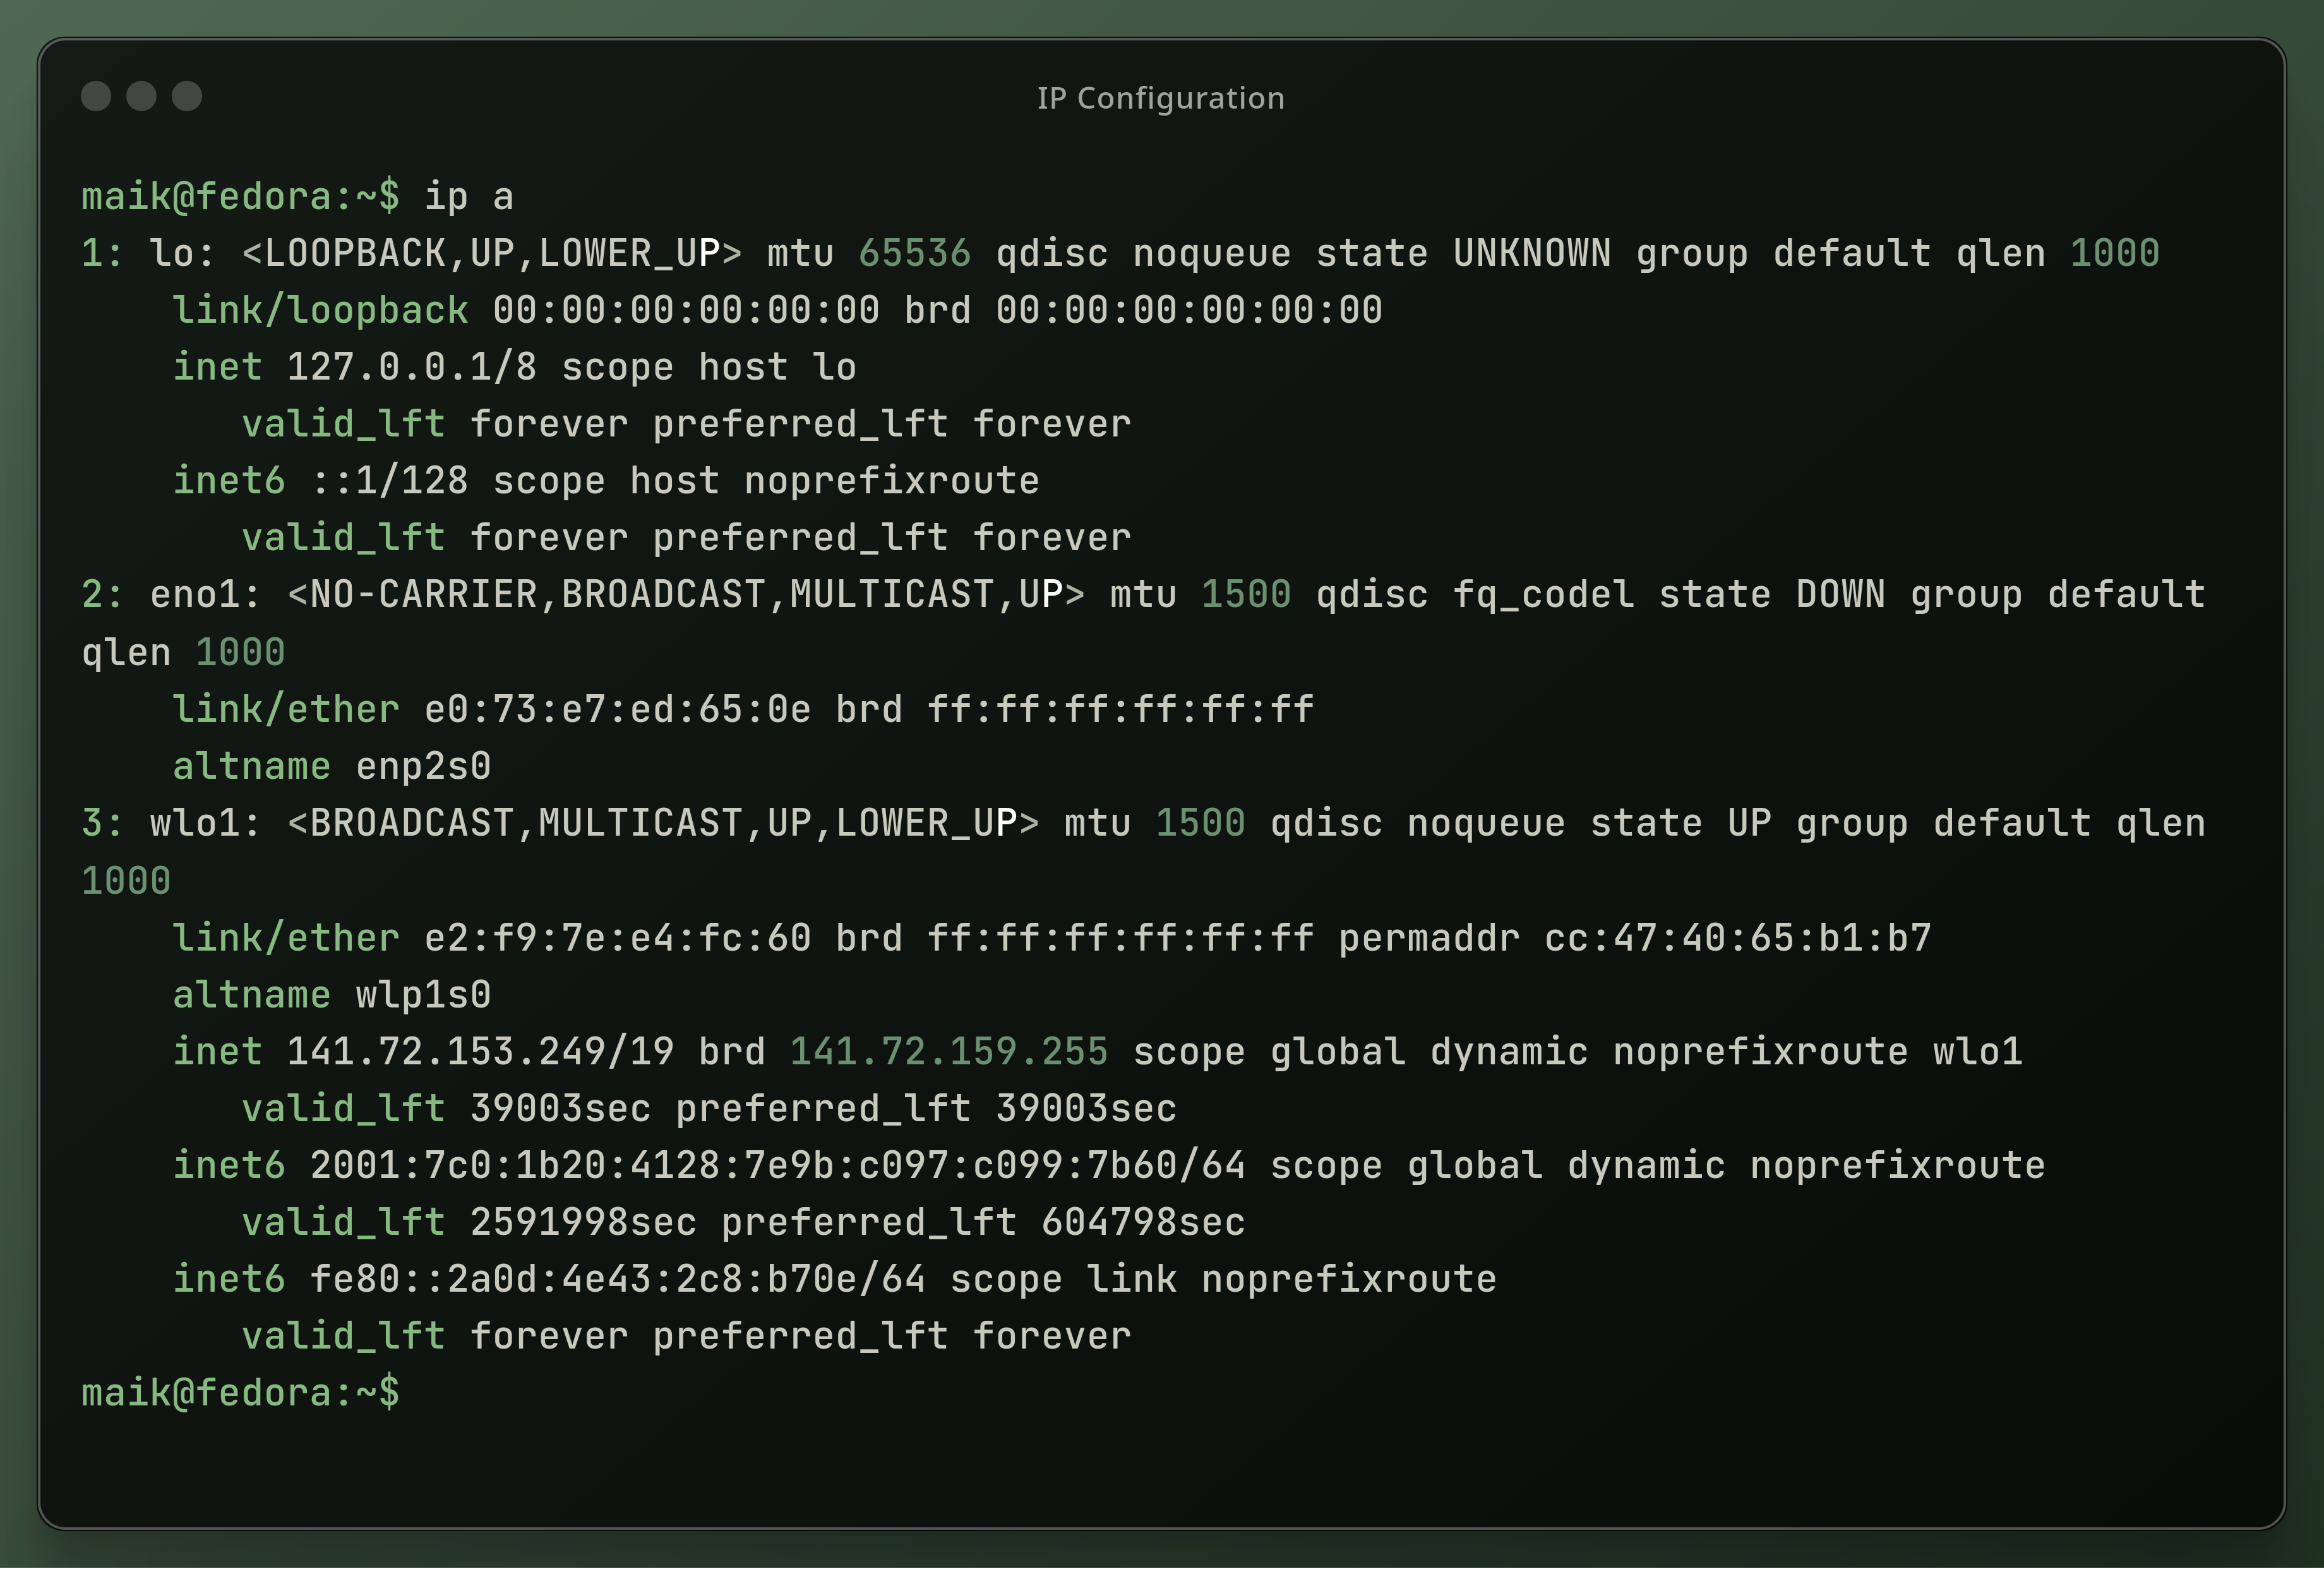
\includegraphics[height=11cm]{ip-configuration}
\end{aufgabe}
\newpage
\begin{aufgabe}
  Öffnen Sie https://ipaddress.com und schauen Sie, ob Ihre IP-Adresse übereinstimmt oder nicht.

  \centering
  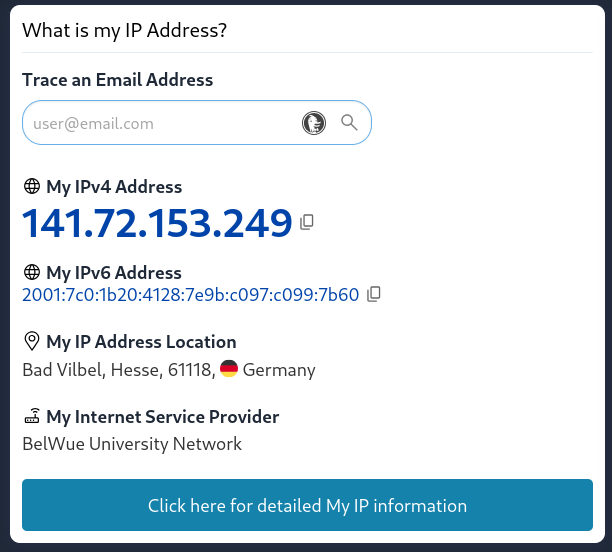
\includegraphics[width=11cm]{ip-address.png}
\end{aufgabe}

\begin{aufgabe}
  Führen Sie den Befehlt \texttt{ping www.google.com} in Ihrer Shell aus. Was kommt dabei heraus?

  \centering
  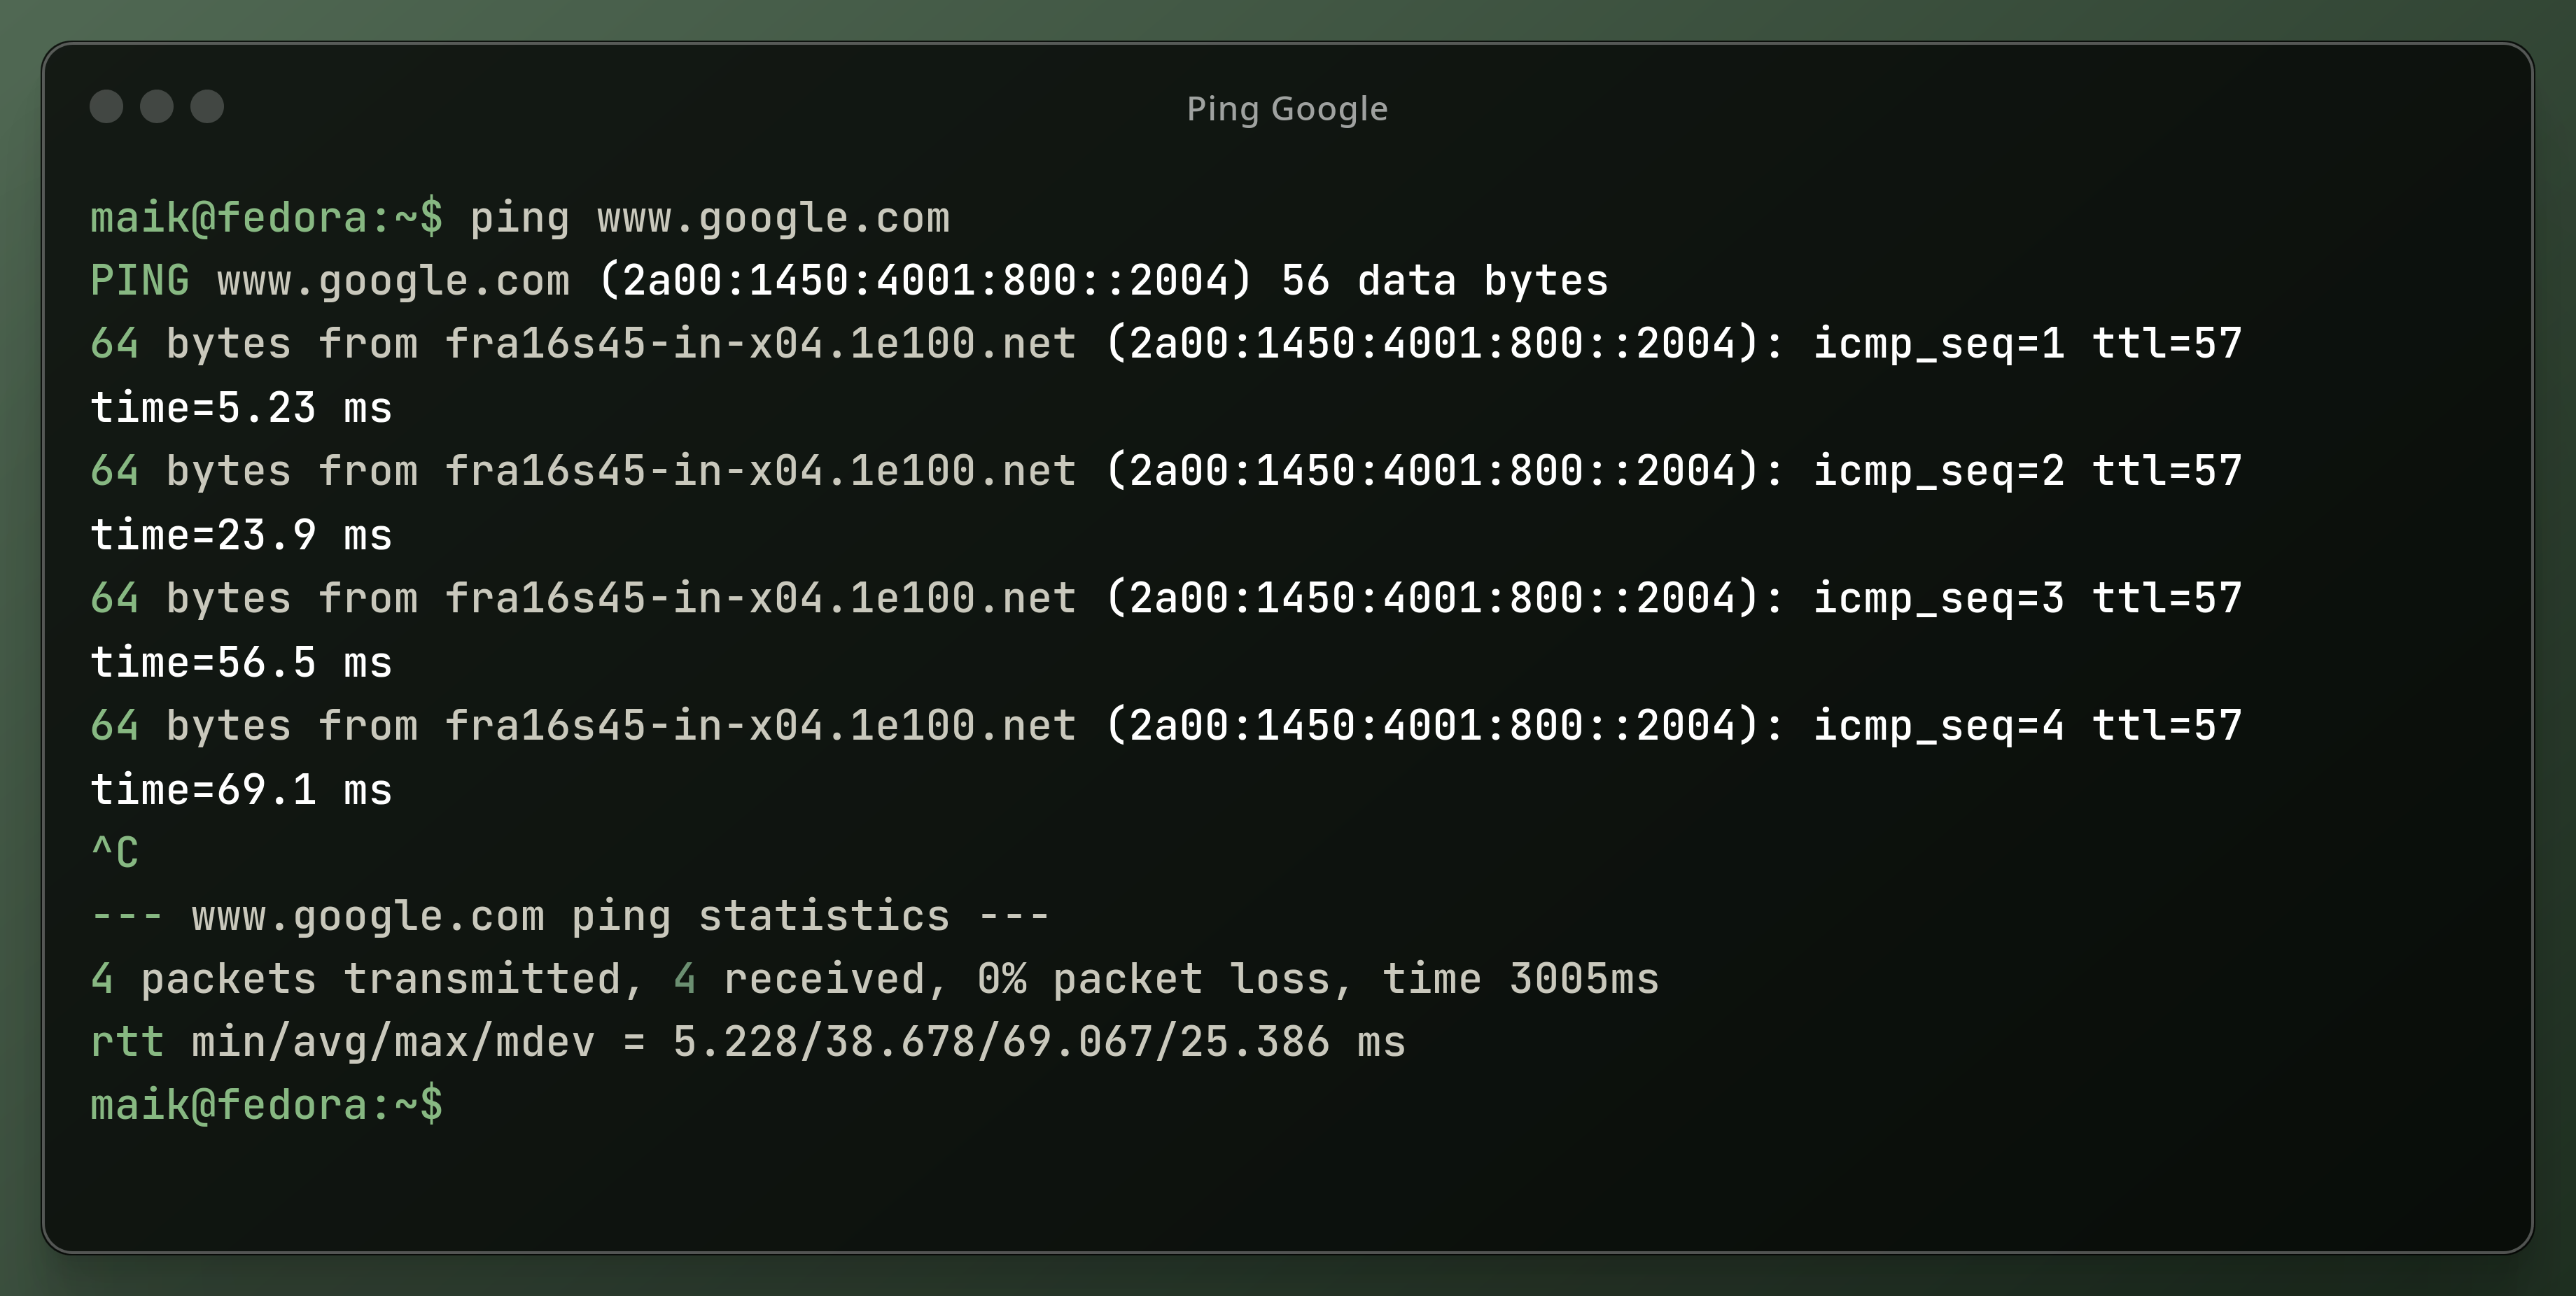
\includegraphics[height=8.5cm]{google-ping.png}
\end{aufgabe}

\begin{aufgabe}
  Schauen Sie sich im StGB-Paragraph §202c an und geben Sie den Inhalt in eigenen Worten wieder.

  Der Artikel beschreibt, dass die Erstellung und Nutzung von Programmen, mit denen Passwörter und andere Zugangscodes
  abgefangen werden können, mit bis zu zwei Jahren Gefängnis bestraft werden können.
\end{aufgabe}

\begin{aufgabe}
  Führen Sie den Befehlt \texttt{traceroute <hostname>} in Ihrer Shell aus. Welche Informationen erhalten Sie?

  Der Befehl trackt den Weg, den ein Datenpaket nimmt, um von dem Ausgangs-PC bis zum Ziel zu kommen.
\end{aufgabe}

\section{Übung -- 05.11.2024}
\begin{aufgabe}
  Was ist HTTP?

  HTTP ("Hypertext Transfer Protocol") ist ein stateless Protokoll zur Übertragung von Daten. Es wird insbesondere
  für den Datentransfer im Internet verwendet.
\end{aufgabe}
\begin{aufgabe}
  Was ist ein Webserver? Was ist ein Webclient?

  Ein Webserver stellt einen bestimmten Service bereit. Das können Dokumente sein, aber auch andere Dienste.

  Ein Webclient nimmt diese Dienste in Anspruch, bzw. erfragt Daten von Webserver. Typische Webclients sind Browser, aber
  es gibt auch anderer Formen von Clients, wie z.B. CLI-Tools.

  Die Kommunikation zwischen Client und Server erfolgt über Protokolle (z.B.).
\end{aufgabe}
\begin{aufgabe}
  Schauen Sie sich die Entwicklerwerkzeuge eines Browsers Ihrer Wahl. Welche Funktion finden Sie am hilfreichsten?

  Der Inspector und Netzwerk Tab sind mit am hilfreichsten, da diese beim Designen und Testen der Website. Welche Funktion finden Sie am hilfreichsten?
\end{aufgabe}
\begin{aufgabe}
  Ablauf von Request/Response?

  Client stellt Anfrage, Server antwortet
\end{aufgabe}

\end{document}